\documentclass[10pt,DIV16,a4paper,abstract=true,twoside=semi,openright]{scrreprt}
\usepackage[english]{babel}
\usepackage[numbers, sort&compress]{natbib}
\usepackage{isabelle,isabellesym}
\usepackage{booktabs}
\usepackage{paralist}
\usepackage{graphicx}
\usepackage{amssymb}
\usepackage{xspace}
\usepackage{xcolor}
\usepackage{hyperref}

\usepackage{enumitem} % Mess about with itemize, enumerate, description styles
\newcommand\mydescriptionlabel[1]{\hspace{\leftmargini}\textbf{#1}}
\newenvironment{where}{%
  \let\descriptionlabel\mydescriptionlabel
  \description[itemsep=0em, font=\normalfont]
}{%
  \enddescription
}


\pagestyle{headings}
\isabellestyle{default}
\setcounter{tocdepth}{1}
\newcommand{\ie}{i.\,e.\xspace}
\newcommand{\eg}{e.\,g.\xspace}
\newcommand{\thy}{\isabellecontext}
\renewcommand{\isamarkupsection}[1]{%
  \begingroup%
  \def\isacharunderscore{\textunderscore}%
  \section{#1 (\thy)}%
  \endgroup%
}

\newcommand{\orcidID}[1]{} % temp. hack

\newcommand{\repeatisanl}[1]
{\ifnum#1=0\else\isanewline\repeatisanl{\numexpr#1-1}\fi}
\newcommand{\snip}[4]{\repeatisanl#2#4\repeatisanl#3}

 \newcommand{\DefineSnippet}[2]{%
   \expandafter\newcommand\csname snippet--#1\endcsname{%
     \begin{quote}
     \begin{isabelle}
     #2
     \end{isabelle}
     \end{quote}}}
 \newcommand{\Snippet}[1]{%
   \ifcsname snippet--#1\endcsname{\csname snippet--#1\endcsname}%
   \else+++++++ERROR: Snippet ``#1 not defined''+++++++ \fi}

\title{A Formal Model of Extended Finite State Machines}%
\author{%
\begin{minipage}{.8\textwidth}
  \centering
      Michael~Foster\footnotemark[1]\orcidID{0000-0001-8233-9873}%
      \qquad\qquad%
      Achim~D.~Brucker\footnotemark[2]\orcidID{0000-0002-6355-1200}%
      \\%
      Ramsay~G.~Taylor\footnotemark[1]\orcidID{0000-0002-4036-7590}%
      \qquad\qquad%
      John~Derrick\footnotemark[1]\orcidID{0000-0002-6631-8914}%
     \end{minipage}
}

\publishers{%
  \footnotemark[1]~Department of Computer Science, The University of Sheffield, Sheffield, UK\texorpdfstring{\\}{, }%
  \texttt{\{%
  	\href{mailto:jmafoster1@sheffield.ac.uk}{jmafoster1},%
  	\href{mailto:r.g.taylor@sheffield.ac.uk}{r.g.taylor},%
  	\href{mailto:j.derrick@sheffield.ac.uk}{j.derrick}%
    \}@sheffield.ac.uk}\\[2em]%
  \footnotemark[2]~%
  Department of Computer Science, University of Exeter, Exeter, UK\texorpdfstring{\\}{, }%
  \href{mailto:a.brucker@exeter.ac.uk}{\texttt{a.brucker@exeter.ac.uk}}%
}

\begin{document}
\maketitle
\begin{abstract}
  In this AFP entry, we provide a formalisation of extended finite state machines (EFSMs) where models are represented as finite sets of transitions between states. EFSMs execute traces to produce observable outputs. We also define various simulation and equality metrics for EFSMs in terms of traces and prove their strengths in relation to each other. Another key contribution is a framework of function definitions such that LTL properties can be phrased over EFSMs. Finally, we provide a simple example case study in the form of a drinks machine.
  \begin{quote}
    \bigskip
    \noindent{\textbf{Keywords:} Extended Finite State Machines, Automata, Linear Temporal Logic}
  \end{quote}
\end{abstract}


\tableofcontents
\cleardoublepage

\chapter{Introduction}
This AFP entry formalises extended finite state machines (EFSMs) as defined in \cite{foster2018}. Here, models maintain both a \emph{control flow state} and a \emph{data state}, which takes the form of a set of \emph{registers} to which values may be assigned. Transitions may take additional input parameters, and may impose guard conditions on the values of both inputs and registers. Additionally, transitions may produce observable outputs and update the data state by evaluating arithmetic functions over inputs and registers.

As defined in \cite{foster2018}, an EFSM is a tuple, $(S, s_0, T)$ where
\begin{where}
  \item [$S$] is a finite non-empty set of states.
  \item [$s_0 \in S$]is the initial state.
  \item [$T$] is the transition matrix $T:(S \times S) \to \mathcal{P}(L \times \mathbb{N} \times G \times F \times U)$ with rows representing origin states and columns representing destination states.
\end{where}
In $T$
\begin{where}
  \item [$L$] is a finite set of transition labels
  \item [$\mathbb{N}$] gives the transition \emph{arity} (the number of input parameters), which may be zero.
  \item [$G$] is a finite set of Boolean guard functions $G:(I \times R) \to \mathbb{B}$.
  \item [$F$] is a finite set of \emph{output functions} $F:(I \times R) \to O$.
  \item [$U$] is a finite set of \emph{update functions} $U:(I \times R) \to R$.
\end{where}
In $G$, $F$, and $U$
\begin{where}
  \item [$I$] is a list $[i_0, i_1, \ldots, i_{m-1}]$ of values representing the inputs of a transition, which is empty if the arity is zero.
  \item [$R$] is a mapping from variables $[r_0, r_1, \ldots]$, representing each register of the machine, to their values.
  \item [$O$] is a list $[o_0, o_1, \ldots, o_{n-1}]$ of values, which may be empty, representing the outputs of a transition.
\end{where}

EFSM transitions have five components: label, arity, guards, outputs, and updates. Transition labels are strings, and the arities natural numbers. Guards have a defined type of \emph{guard expression} (\texttt{gexp}) and the outputs and updates are defined using \emph{arithmetic expressions} (\texttt{aexp}). Outputs are simply a list of expressions to be evaluated. Updates are a list of pairs with the first element being the index of the register to be updated, and the second element being an arithmetic expression to be evaluated.

\begin{figure}
  \centering
  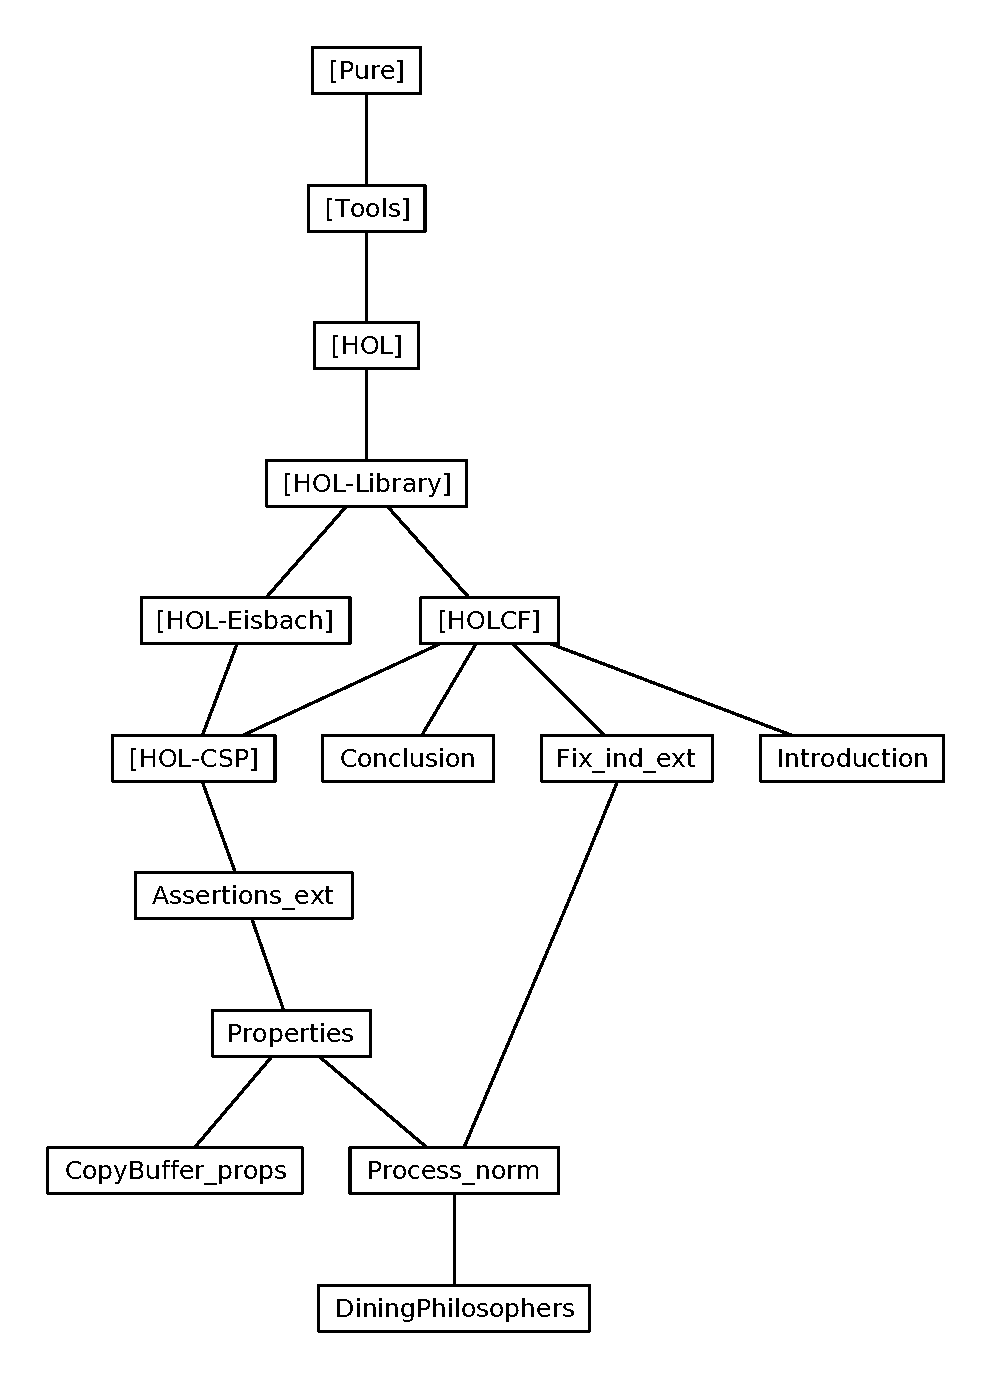
\includegraphics[height=\textheight]{session_graph}
  \caption{The Dependency Graph of the Isabelle Theories.\label{fig:session-graph}}
\end{figure}
The rest of this document is automatically generated from the
formalization in Isabelle/HOL, i.e., all content is checked by
Isabelle.  Overall, the structure of this document follows the
theory dependencies (see \autoref{fig:session-graph}):

\nocite{foster2018}

\clearpage
% \chapter{Theories}

\input{session}


{\small
  \bibliographystyle{abbrvnat}
  \bibliography{root}
}
\end{document}
\endinput
%%% Local Variables:
%%% mode: latex
%%% TeX-master: t
%%% End:
